\documentclass{article}
\usepackage{graphicx}
\usepackage{mathtools}

%\includegraphics[width=\textwidth, trim={0 0 0 6.5in},clip]

\begin{document}

\title{2D Meshless Moving Least Squares Poisson Solver}
\author{Sam Maloney}

\maketitle


\section{The Problem}

The program solves a simple 2D Poisson problem on a unit square domain, specifically the homogeneous equation,
\begin{equation}
-u_{xx}(x,y)-u_{yy}(x,y)=0,\qquad(x,y)\in\Omega=(0,1)\times(0,1),
\end{equation}

\noindent
with Dirichlet boundary conditions given as,
\begin{align}
\begin{split}
u(0,y)=u(1,y)=0,&\qquad0\leq y\leq1,\\
u(x,0)=0,&\qquad0\leq x\leq1,\\
u(x,1)=\sin(k\pi x),&\qquad0<x<1,
\end{split}
\end{align}

\noindent
which has analytic solutions given by,
\begin{equation}
u_k(x,y)=\sin(k\pi x)\sinh(k\pi y).
\end{equation}


\section{The Program}

The numerical solution is computed using linear moving least squares (MLS) shape functions on a set of nodes regularly spaced throughout the unit square domain. Fig.~\ref{fig:points} shows the set of nodes for $N=2$ grid divisions, as well as examples of the possible sets of quadrature points that the code can use, based on the number and distribution of points in each cell of the underlying grid implied by the nodal arrangment. These quadrature points are used for computing the numerical integration required when using the Galerkin method for asembling the stiffness matrix. No integration, and thus no quadrature points, are required when using the collocation assembly method.

\begin{figure}
\centering
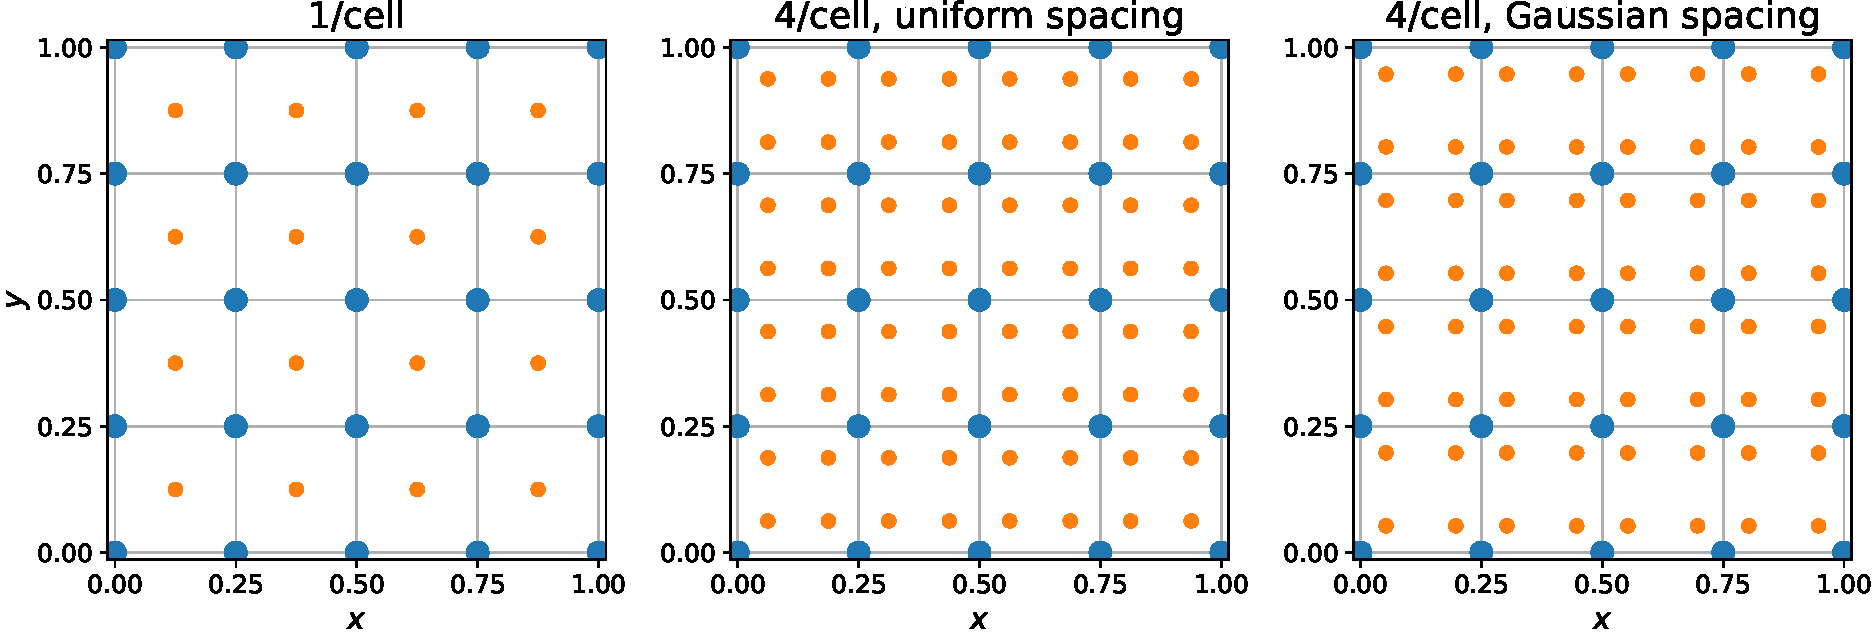
\includegraphics[width=\textwidth]{../coursework-sam-maloney/MLS/MLS_points.pdf}
\caption{Example of the regular set of nodes used for the MLS simulation with $N=2$ grid divisions along each axis. Nodal points where the solution is computed are shown as larger blue points, while quadrature points used for integration in the Galerkin method are shown as smaller orange points}
\label{fig:points}
\end{figure}

The script in \texttt{MlsSim.py} defines an MLS simulation class which is used to generate and store the set of nodes and quadrature points for a given number of grid divisions, and has methods to compute the required shape functions. Other class methods are provided to compute and assemble the stiffness matrix, and some sparse linear algebra routines and iterative solvers from scipy are used to compute the numerical solution for the given set of nodes.

\subsection{Parameters}

There are a number of parameters and options that can be tuned and selected for a given MLS simulation and those currently implemented in my code are the following:

\begin{enumerate}
\item The stiffness matrix assembly method.
	\begin{itemize}
	\item Can use either the Galerkin or collocation methods.
	\item Galerkin method requires integration while collocation does not.
	\end{itemize}
\item The number of quadrature points used per cell.
\item The distribution of those quadrature points within each cell.
	\begin{itemize}
	\item Can use either a uniform spatial distribution or Gauss-Legendre rules.
	\item Gauss-Legendre is currently only specified for 2 points per dimension.
	\end{itemize}
\item The underlying kernel weight functions.
	\begin{itemize}
	\item Either a cubic or a quartic spline function can be selected.
	\end{itemize}
\item The size of the support for the shape functions.
	\begin{itemize}
	\item Currently only circular supports are implemented.
	\item Other shapes (e.g.~squares) are possible for the MLS method.
	\end{itemize}
\end{enumerate}


\section{MLS Shape Functions}

The basic form of the MLS shape functions are shown in Fig.~\ref{fig:shape_functions} for $N=4$ grid divisions and a support radius of 2X the grid spacing, demonstrating the basic symmetries of the shape functions and how they behave both in the interior of the domain and at nodes near the boundary. In particular, one can see how the fully interior shape function ($\Phi_{12}$) is symmetric in both $x$ and $y$, but all the other shape functions become squashed as they near the boundary, where their full region of support would otherwise extend to areas outside of the domain. Looking at the colorbar limits we can see that the maximal values of the inidividual shape functions are also much higher near the boundaries than in the interior since they must form a partition of unity, i.e.~there are less shape functions whose support includes points near the boundary so those shape functions that do cover such points must have correspondingly larger values in those areas to ensure that the full sum over all shape functions still adds up to unity.

\begin{figure}
\centering
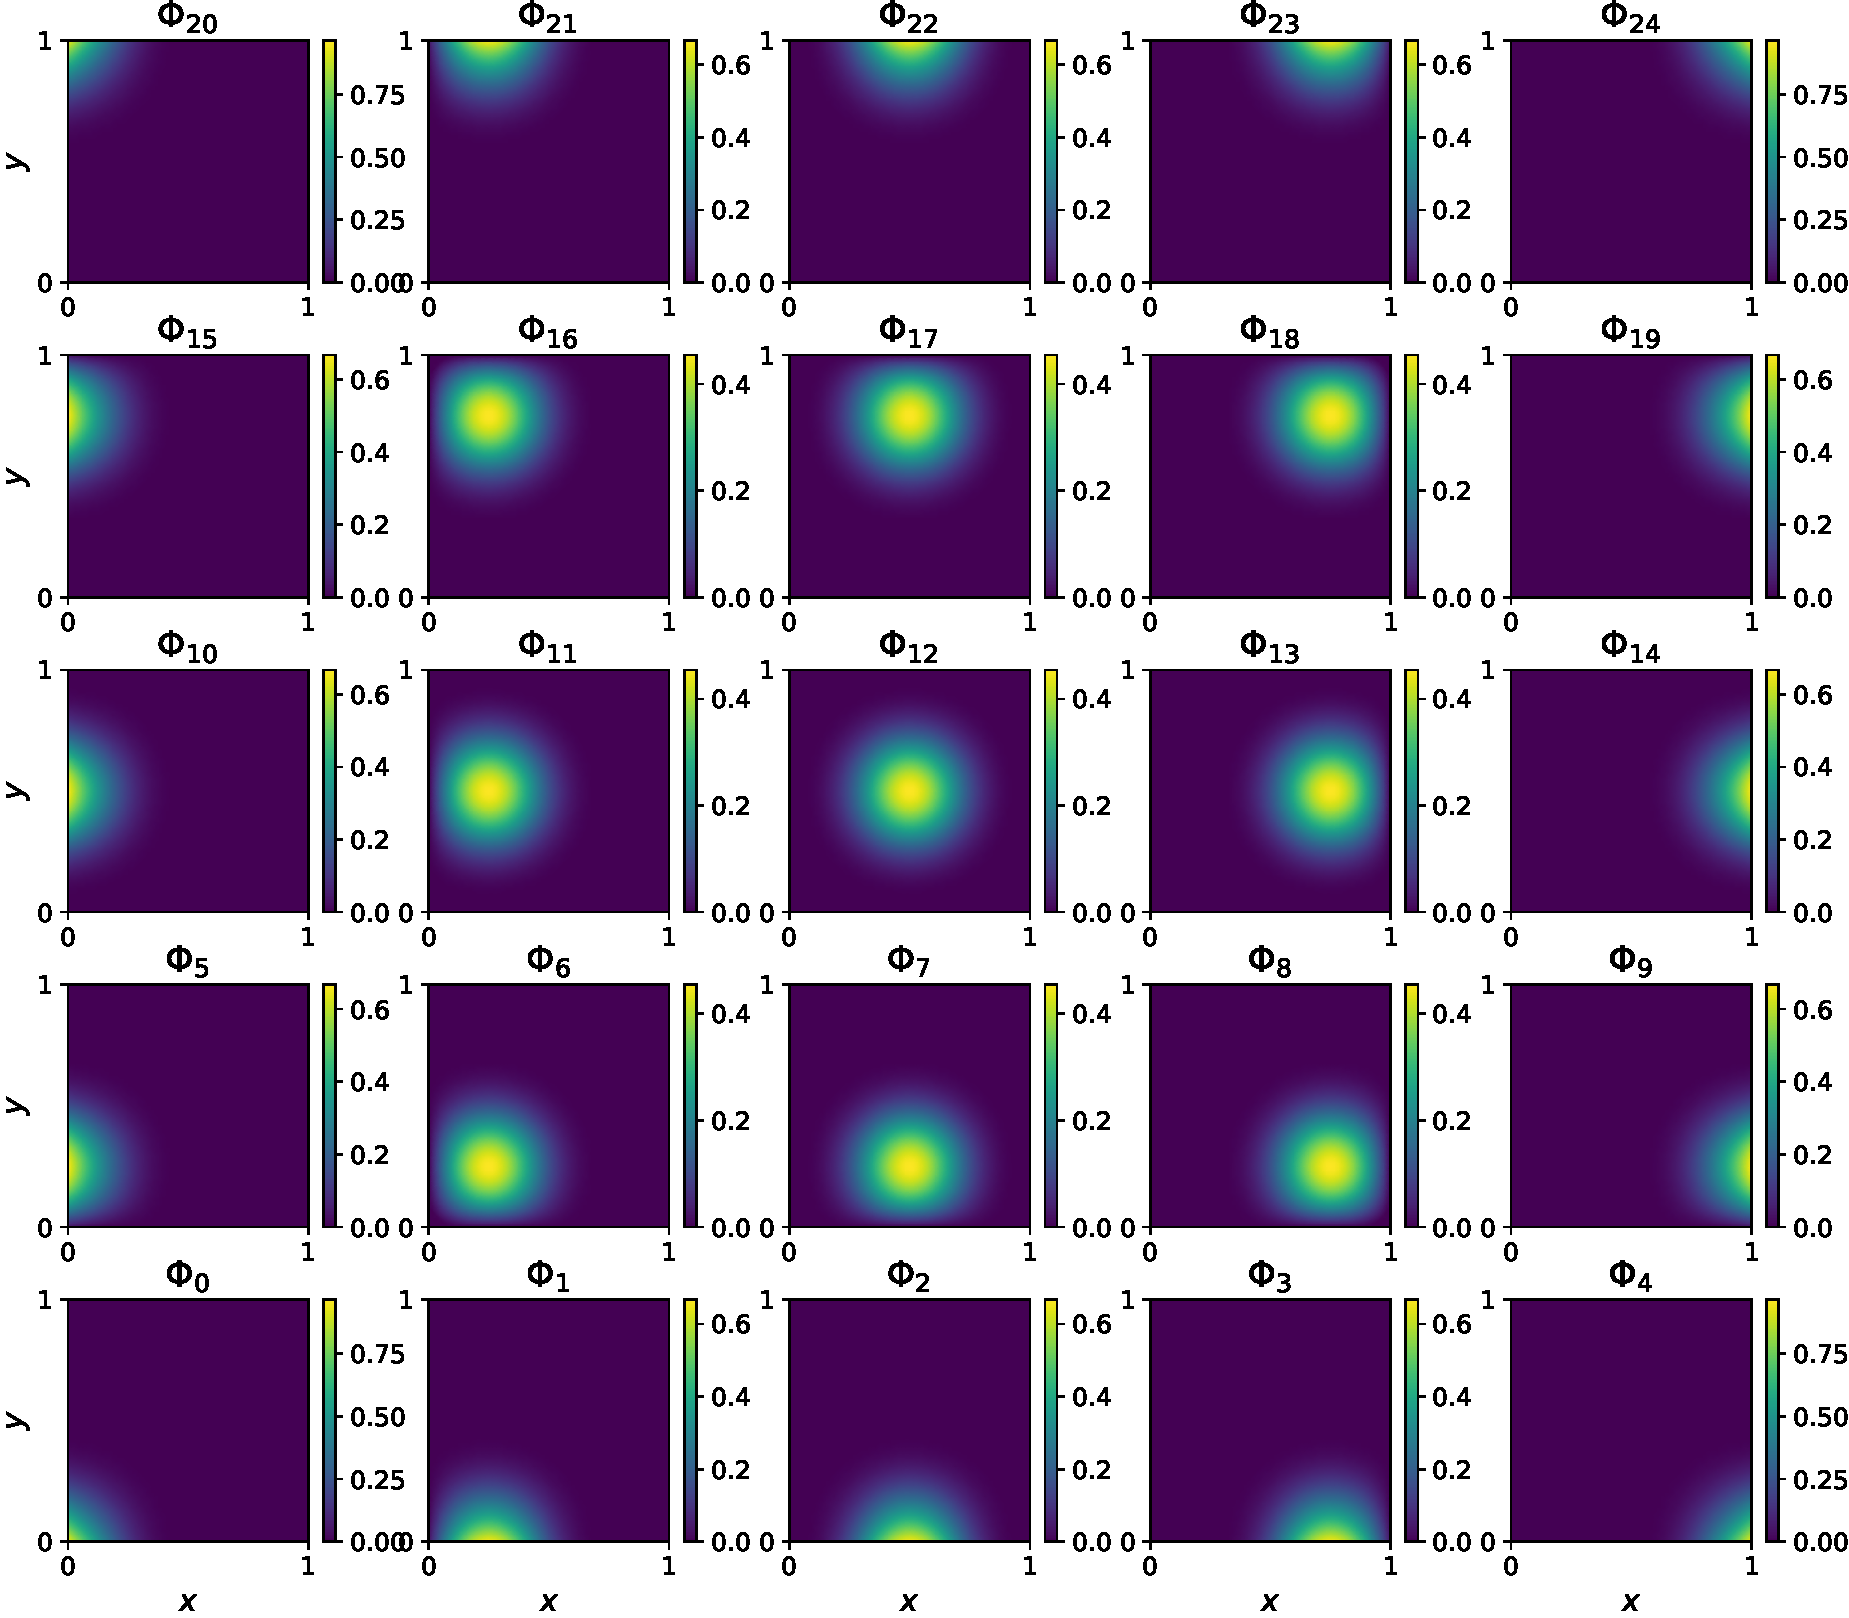
\includegraphics[width=\textwidth]{{../coursework-sam-maloney/MLS/MLS_shape_functions5}.pdf}
\caption{MLS shape functions for $N=4$ grid divisions and support radius of 2X the grid spacing. Note that not all colorbars have the same upper limits (they do all have a minimum of zero), so mapping of values to colors is not identical between all plots.}
\label{fig:shape_functions}
\end{figure}

\subsection{Representation of other functions}

Since these MLS shape functions are based on the set of linear basis functions $[1 x y]$ they should be able to represent constanst functions and first-order polynomials exactly. We can see this demonstrated in Fig.~\ref{fig:func_one} for a constant unity function $f(x,y)=1$ and Fig.~\ref{fig:func_xpy} for a plane surface $f(x,y)=x+y$. Results shown are for $N=8$ grid divisions, but the machine precision accuracy is maintained for any number of supplied shape functions down to $N=1$, thus illustrating the partition of unity property for the set of MLS shape functions and the exact representation of first-order polynomials.

\begin{figure}
\centering
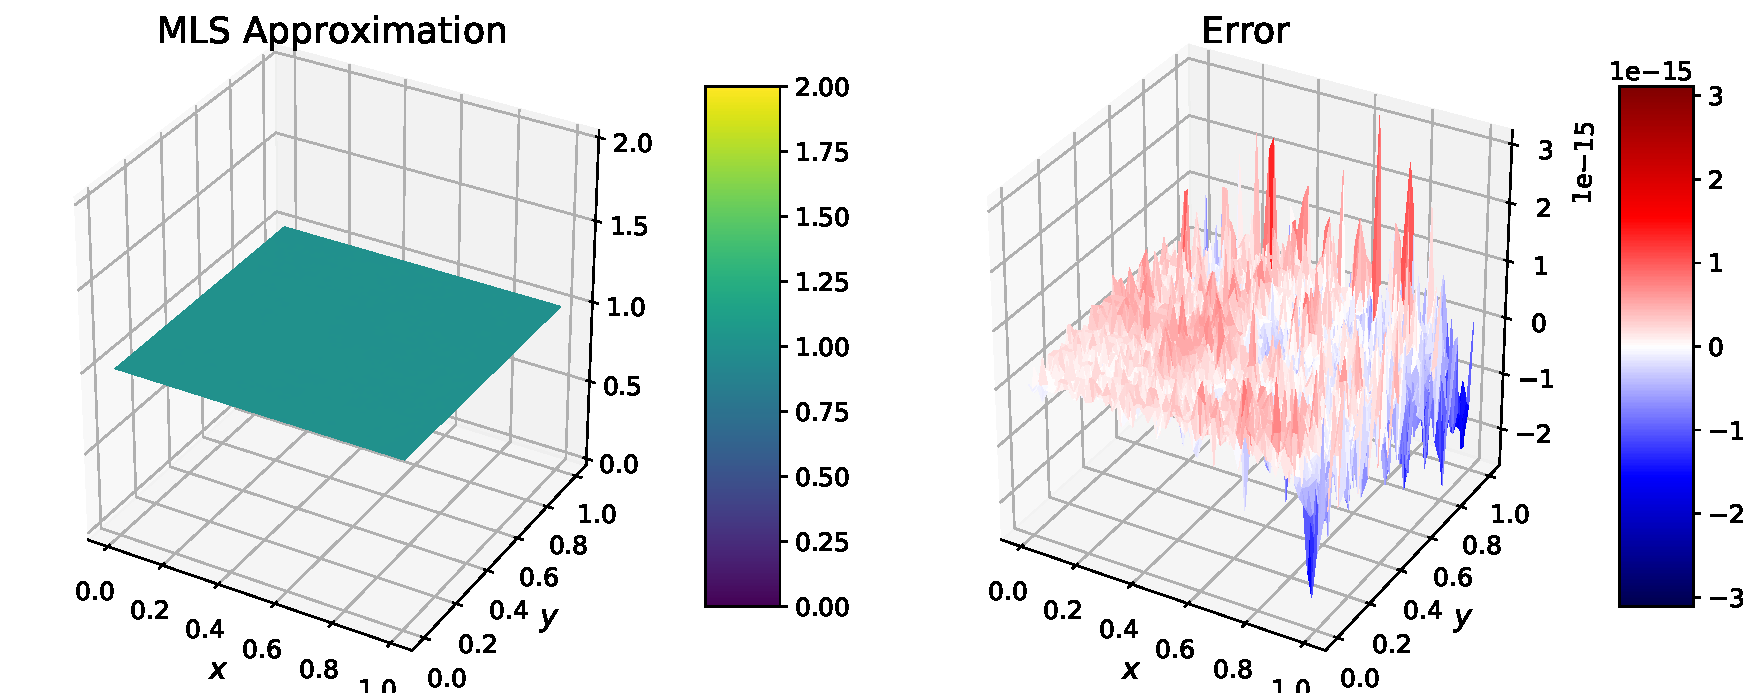
\includegraphics[width=\textwidth]{{../coursework-sam-maloney/MLS/MLS_one}.pdf}
\caption{Representation of a constant unity function $f(x,y)=1$ using MLS shape functions and $N=8$ grid divisions.}
\label{fig:func_one}
\end{figure}

\begin{figure}
\centering
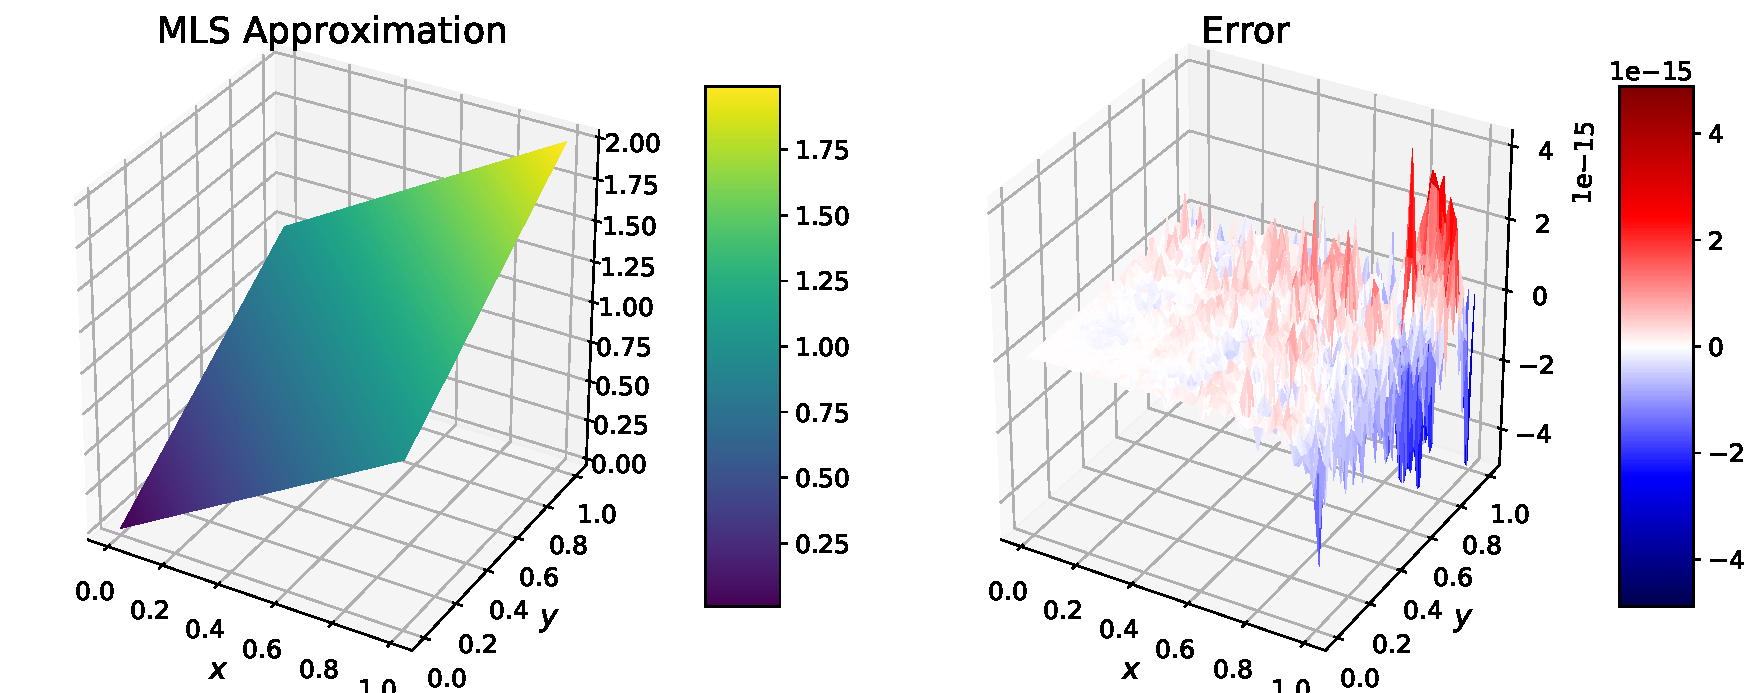
\includegraphics[width=\textwidth]{{../coursework-sam-maloney/MLS/MLS_xpy}.pdf}
\caption{Representation of a planar surface $f(x,y)=x+y$ using MLS shape functions and $N=8$ grid divisions.}
\label{fig:func_xpy}
\end{figure}

And as can be seen in Fig.~\ref{fig:func_x2} for $f(x,y)=x^2$, as soon as one moves to higher order polynomials the representation then has some finite error, and as would be expected for a convex function the linear basis consistently overestimates its value. Lastly, in Fig.~\ref{fig:func_sinxpy} is shown the representation of $f(x,y)=\sin(x+y)$, again showing the over- and under-estimation of the function in areas of convexity and concavity, respectively.

\begin{figure}
\centering
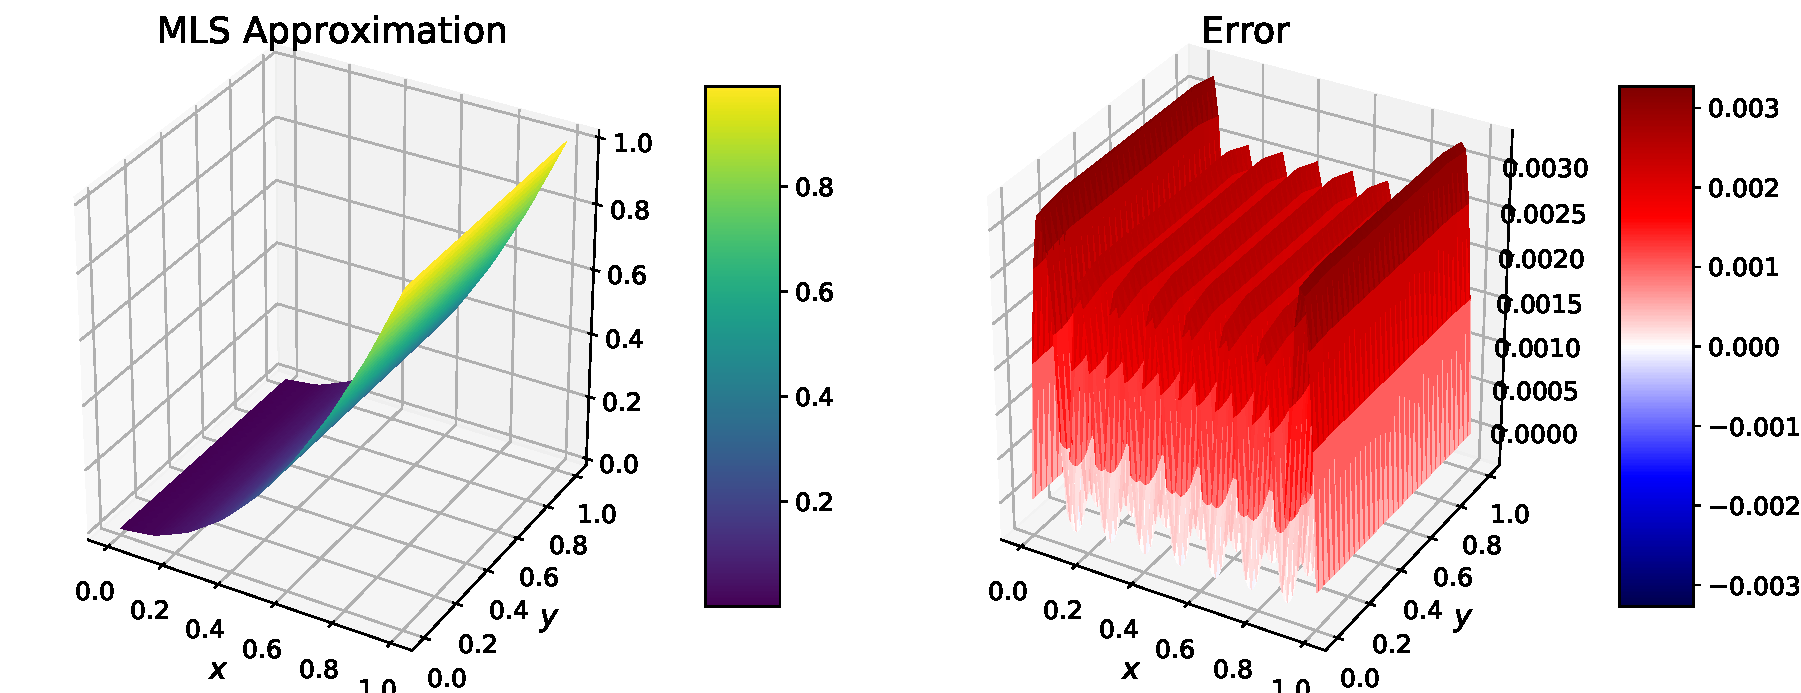
\includegraphics[width=\textwidth]{{../coursework-sam-maloney/MLS/MLS_x2}.pdf}
\caption{Representation of a quadratic function $f(x,y)=x^2$ using MLS shape functions and $N=8$ grid divisions.}
\label{fig:func_x2}
\end{figure}

\begin{figure}
\centering
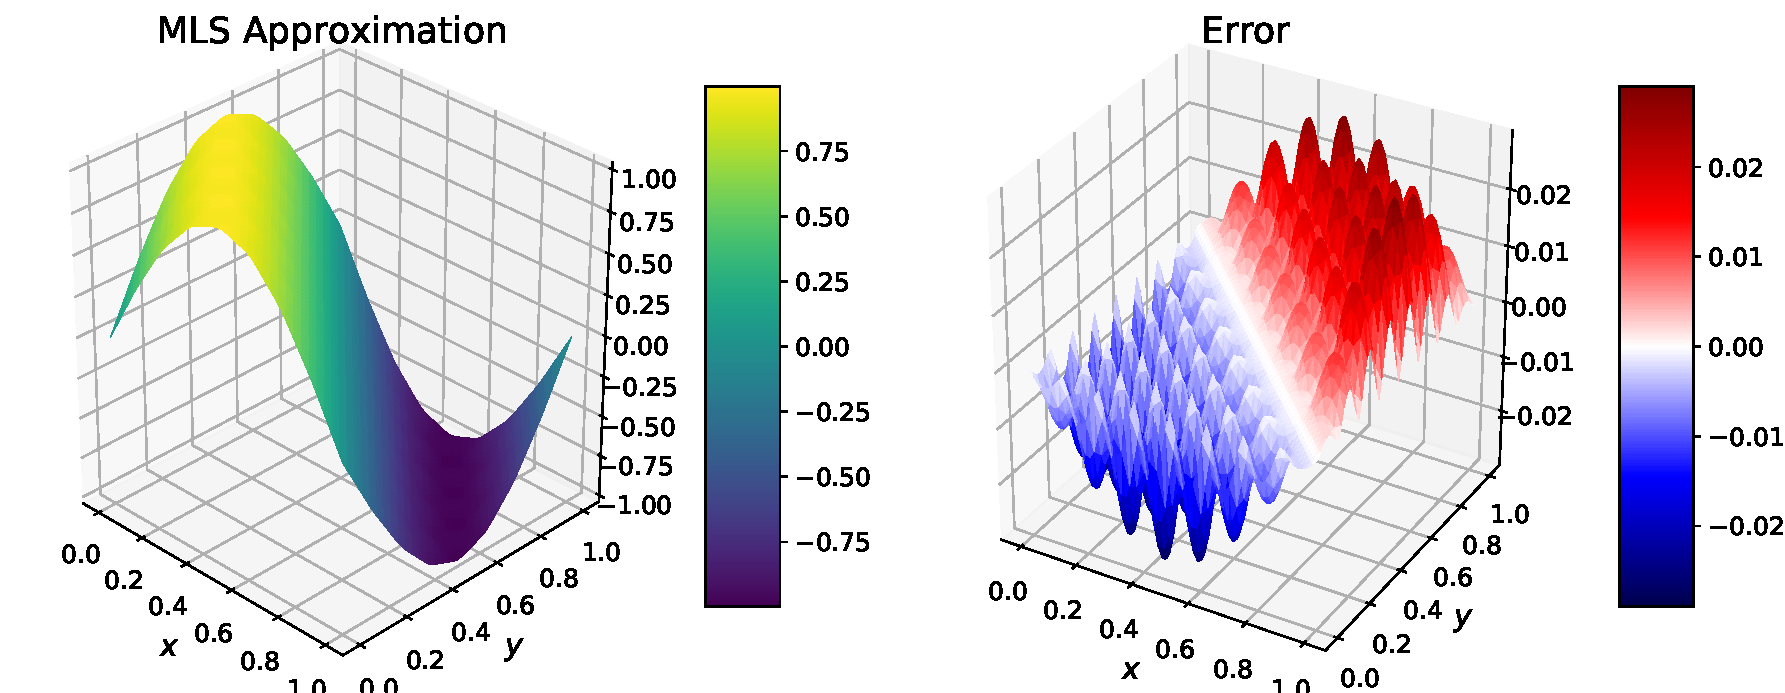
\includegraphics[width=\textwidth]{{../coursework-sam-maloney/MLS/MLS_sinxpy}.pdf}
\caption{Representation of a sinusoidal surface $f(x,y)=\sin(x+y)$ using MLS shape functions and $N=8$ grid divisions.}
\label{fig:func_sinxpy}
\end{figure}


\section{Parameter Comparisons}

\subsection{Convergence Testing}

To test convergence of the method for a given set of parameters, a loop over the number of grid divisions is performed, doubling each time, such that the convergence of the numerical solution towards the expected analytic result can be observed. These convergence tests were repeated for various combinations of the available input parameters and stiffness matrix assembly methods to compare the performance of each. The $E_2$ and $E_\infty$ error norms are computed, corresponding to the Euclidean norm of the error normalized by the number of grid divisions and the maximum absolute error, respectively.

\subsection{Galerkin vs. Collocation Assembly and Cubic vs. Quartic Splines}

In Fig.~\ref{fig:timings_method_form_1k} is a summary of results comparing the Galerkin and collocation assembly methods, as well as the cubic and quartic spline kernel weighting functions. All Galerkin assembly was performed with a single quadrature point per cell.

Looking at the error magnitudes we can immediately see that the Galerkin method far outperforms the collocation method for all tests, the reason for which is most clearly seen in matrix condition numbers, where the collocation method produces very ill-conditioned stiffness matrices for all support sizes tested, while the Galerkin method gives relatively well-posed systems for a range of smaller support sizes. It should be noted that these are the smalest support sizes possible for this problem set-up, as going any smaller means there would not be enough overlap between the shape functions to give a non singular moment matrix when computing the shape functions.

\begin{figure}
\centering
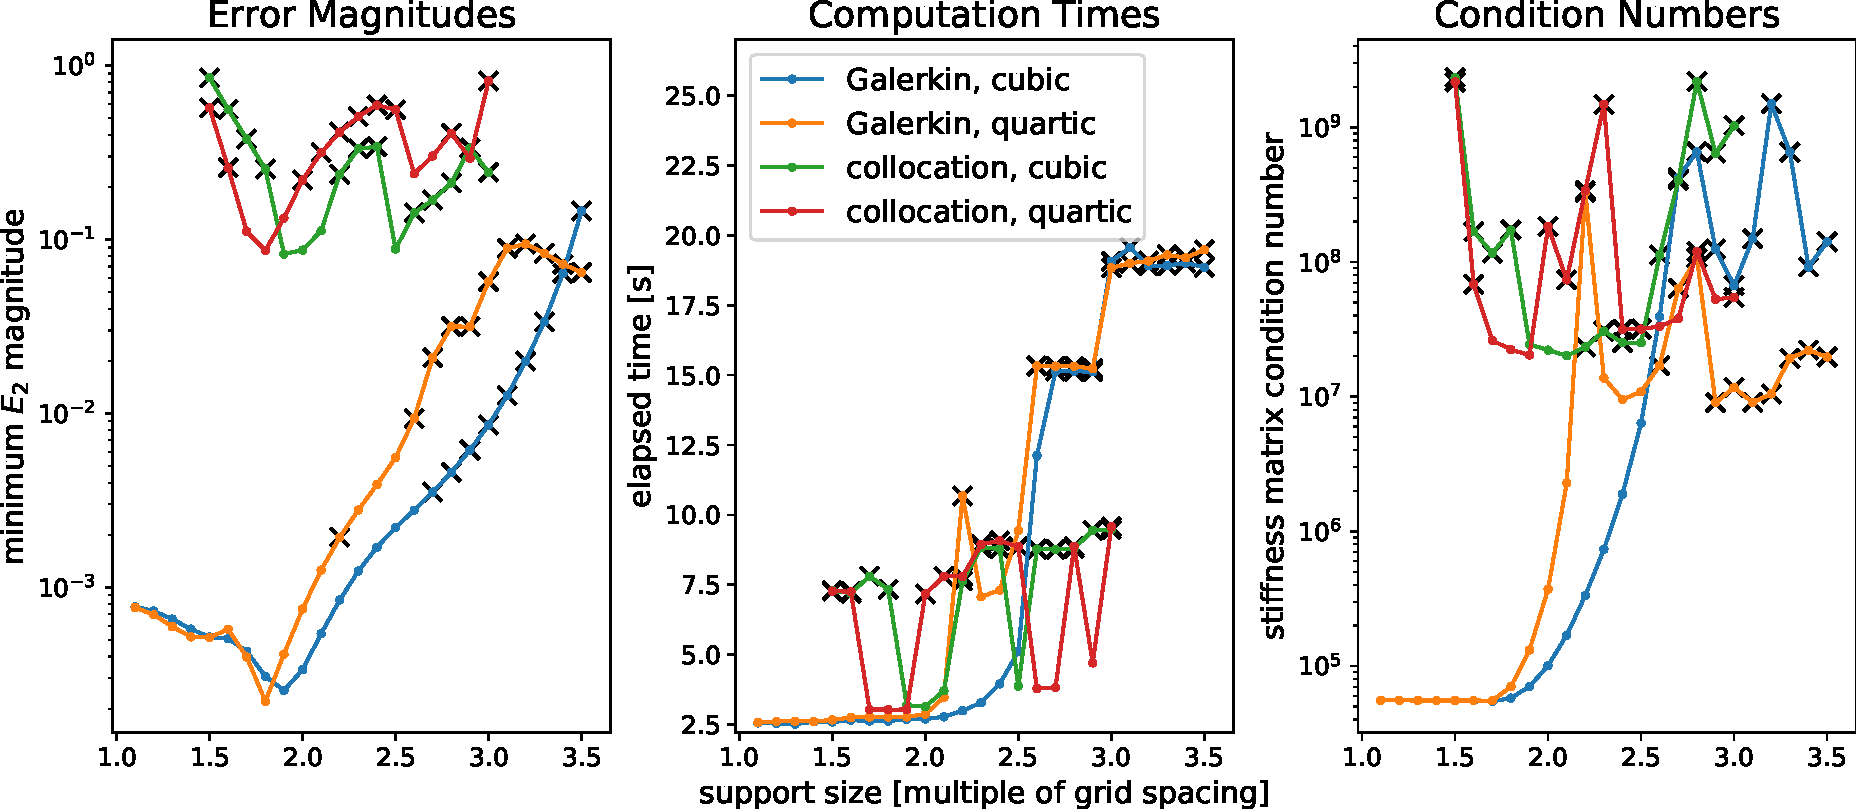
\includegraphics[width=\textwidth]{{../coursework-sam-maloney/MLS/MLS_timings_method_form_1k}.pdf}
\caption{Comparison of minimum errors, simulation wall timings, and stiffness matrix condition numbers between the Galerkin and collocation assembly methods using both cubic and quartic spline kernel functions. All timings and condition numbers are for $N=64$ grid divisions, and errors are the minimum $E_2$ error norm values achieved during a convergence study from $N=2$ to $N=64$ grid divisions. Black $\times$'s indicate data points where the \texttt{lgmres} solver did not converge after $1000$ iterations for the $N=64$ case.}
\label{fig:timings_method_form_1k}
\end{figure}

\begin{figure}[!ht]
\centering
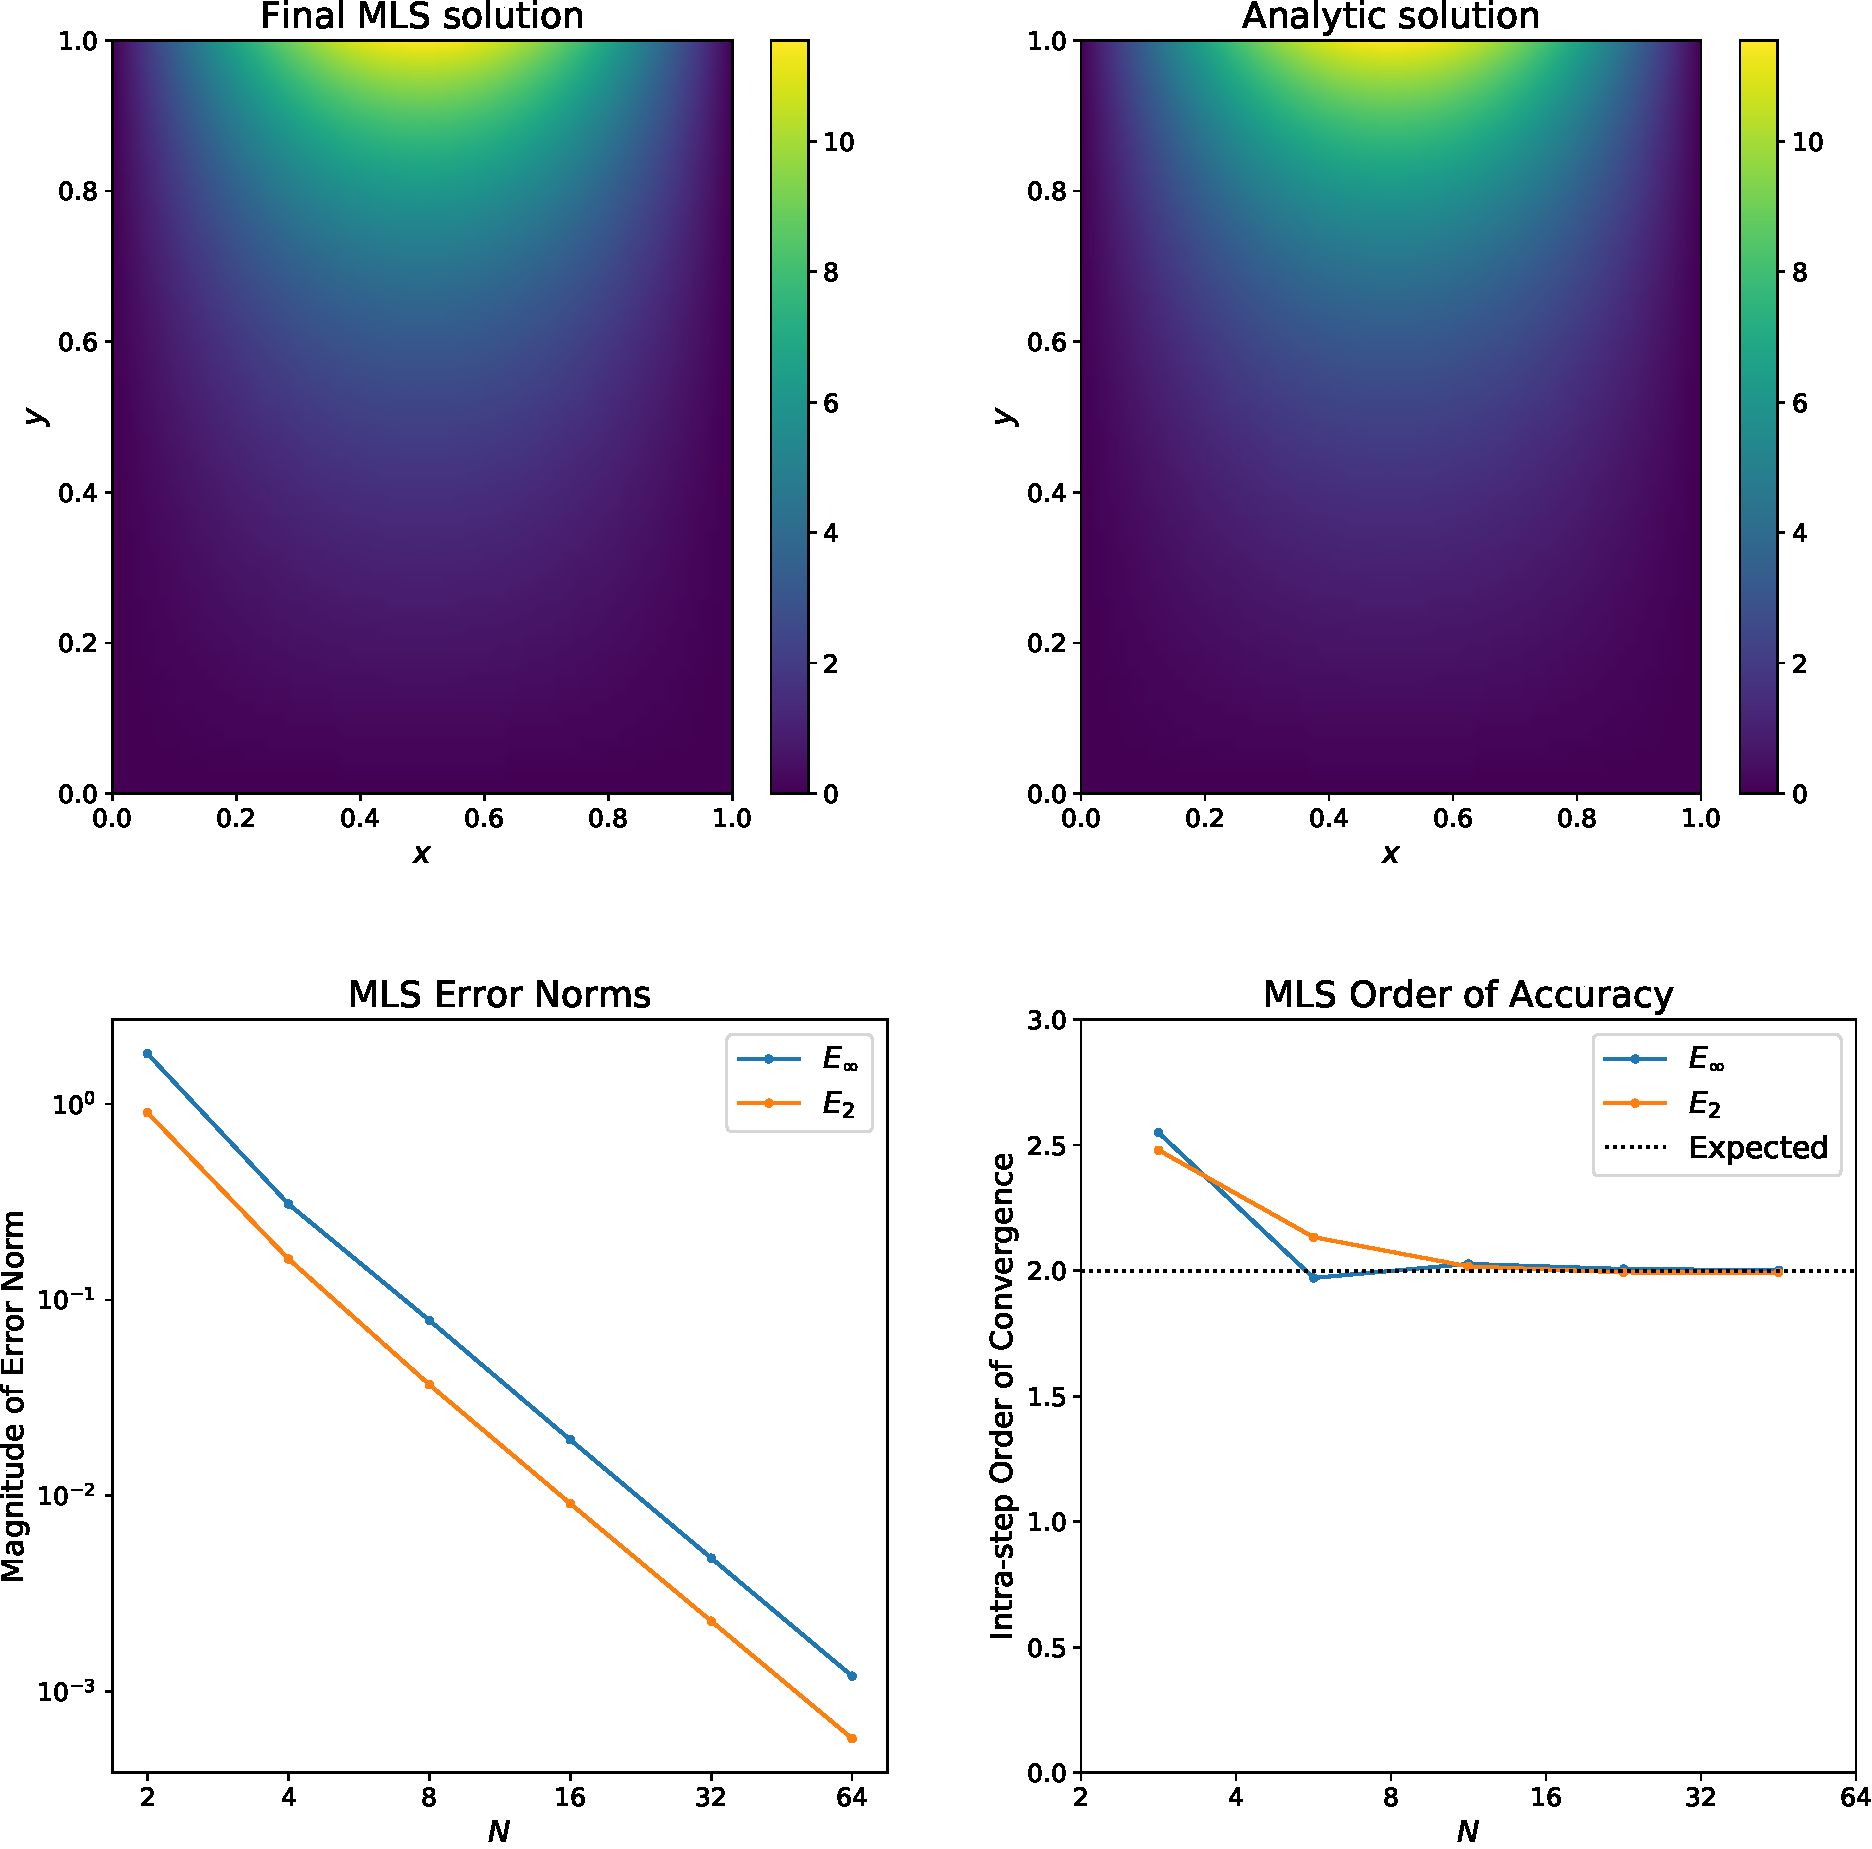
\includegraphics[width=\textwidth]{{../coursework-sam-maloney/MLS/MLS_galerkin_cubic_1k_1Q_1.4S}.pdf}
\caption{Final results of the MLS simulation compared to the expected analytic solution, and convergence study showing desired 2nd order spatial accuracy. Simulation used Galerkin assembly, cubic splines, 1 quadrature point per cell, and a support radius of 1.4X the grid spacing.}
\label{fig:G_c_1_1_1.4}
\end{figure}

In terms of convergence, we can see an example of a well-converged Galerkin solution in Fig.~\ref{fig:G_c_1_1_1.4} side by side with the analytic solution for visual comparison, as well as plots of the error norms and order of convergence to validate the expected 2nd order spatial accuracy of the method. Conversely, we can see in Fig.~\ref{fig:C_c_1_1_1.8} the results of a convergence study using the collocation method, where even though this is the parameter set with the lowest error of all the collocation simulations (cubic splines and support radius of 1.8X the grid spacing) no convergence towards the analytic solution is observed, and the higher resolution simulations simply lead to spurious oscillatory states that do not respect the imposed Dirichlet boundary conditions at the top edge of the domain.

\begin{figure}
\centering
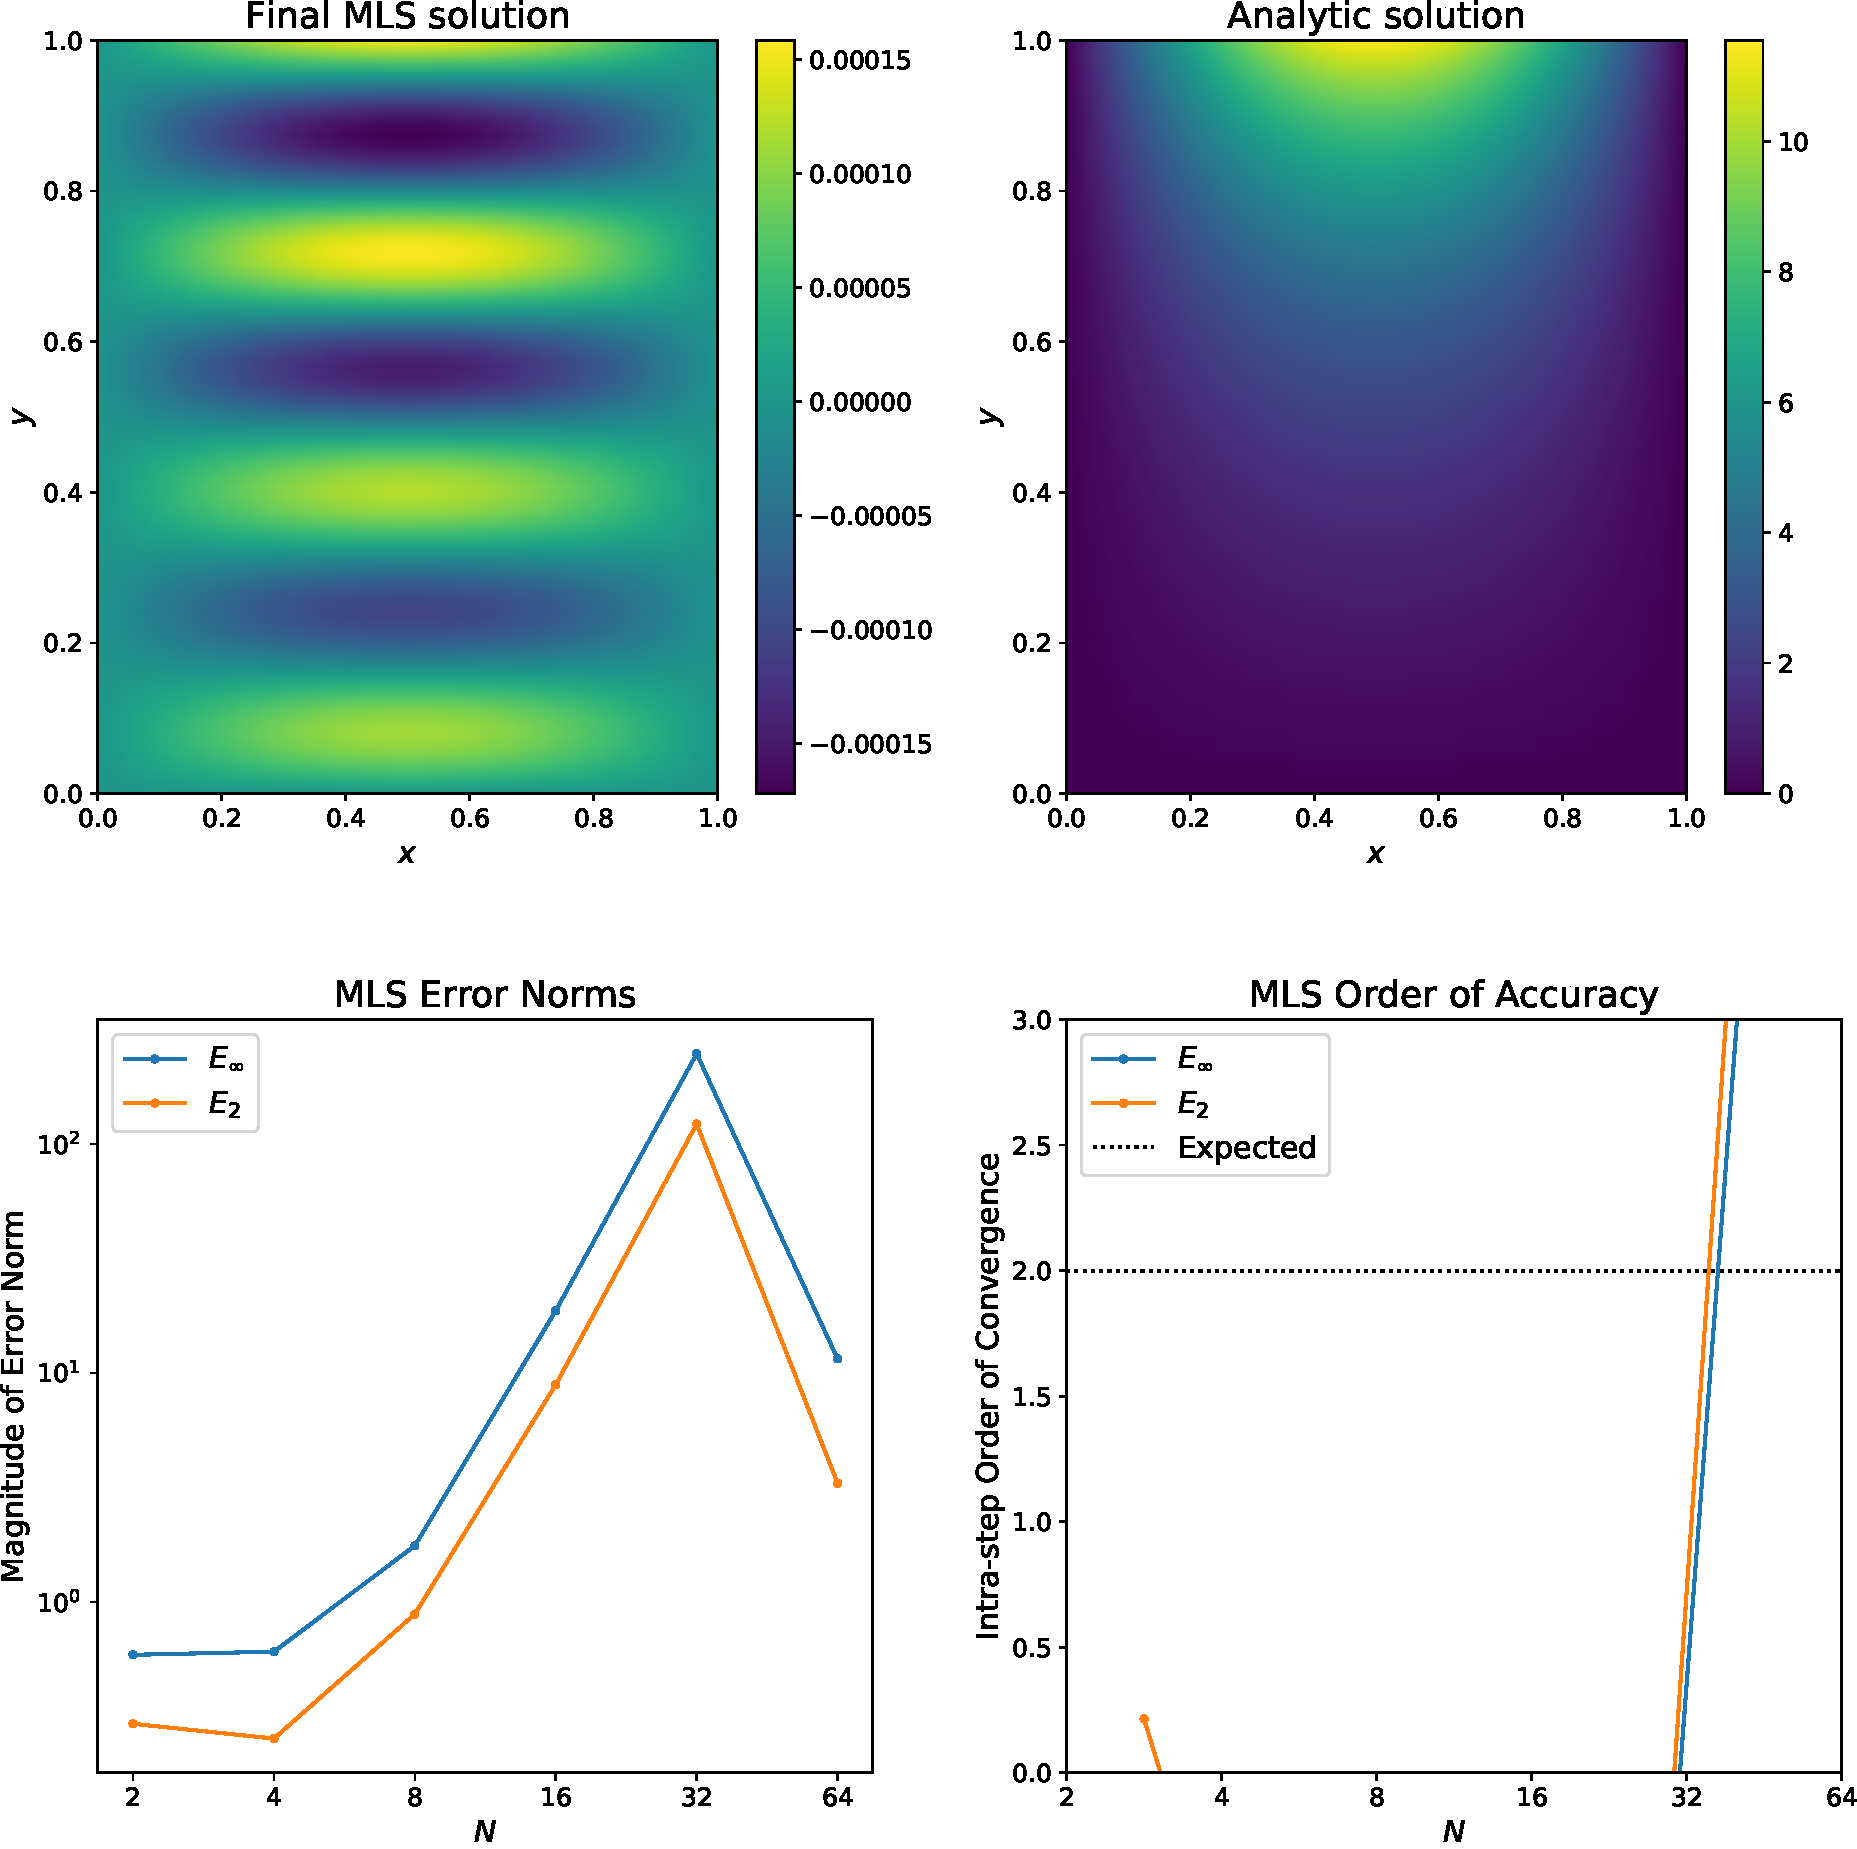
\includegraphics[width=\textwidth]{{../coursework-sam-maloney/MLS/MLS_collocation_cubic_1k_1Q_1.8S}.pdf}
\caption{Final results of the MLS simulation compared to the expected analytic solution, and convergence study not showing desired 2nd order spatial accuracy. Simulation used collocation assembly, cubic splines, and a support radius of 1.8X the grid spacing.}
\label{fig:C_c_1_1_1.8}
\end{figure}

Overall the cubic spline kernel weight function seems to outperform the quartic spline, although the differences are quite marginal over the rane of supports for which the condition number and error of the systems is lowest, so the choice is relatively arbitrary. Computation times as well are quite similar for the parameter sets that led to good solutions, differing mostly only at larger support radii for which the system become more ill-conditioned.

\subsection{Number and distribution of quadrature points}

In Fig.~\ref{fig:timings_quadrature_1k} is a summary of results comparing the quadrature options for the Galerkin assembly method, using cubic splines for the kernel weighting functions.

\begin{figure}
\centering
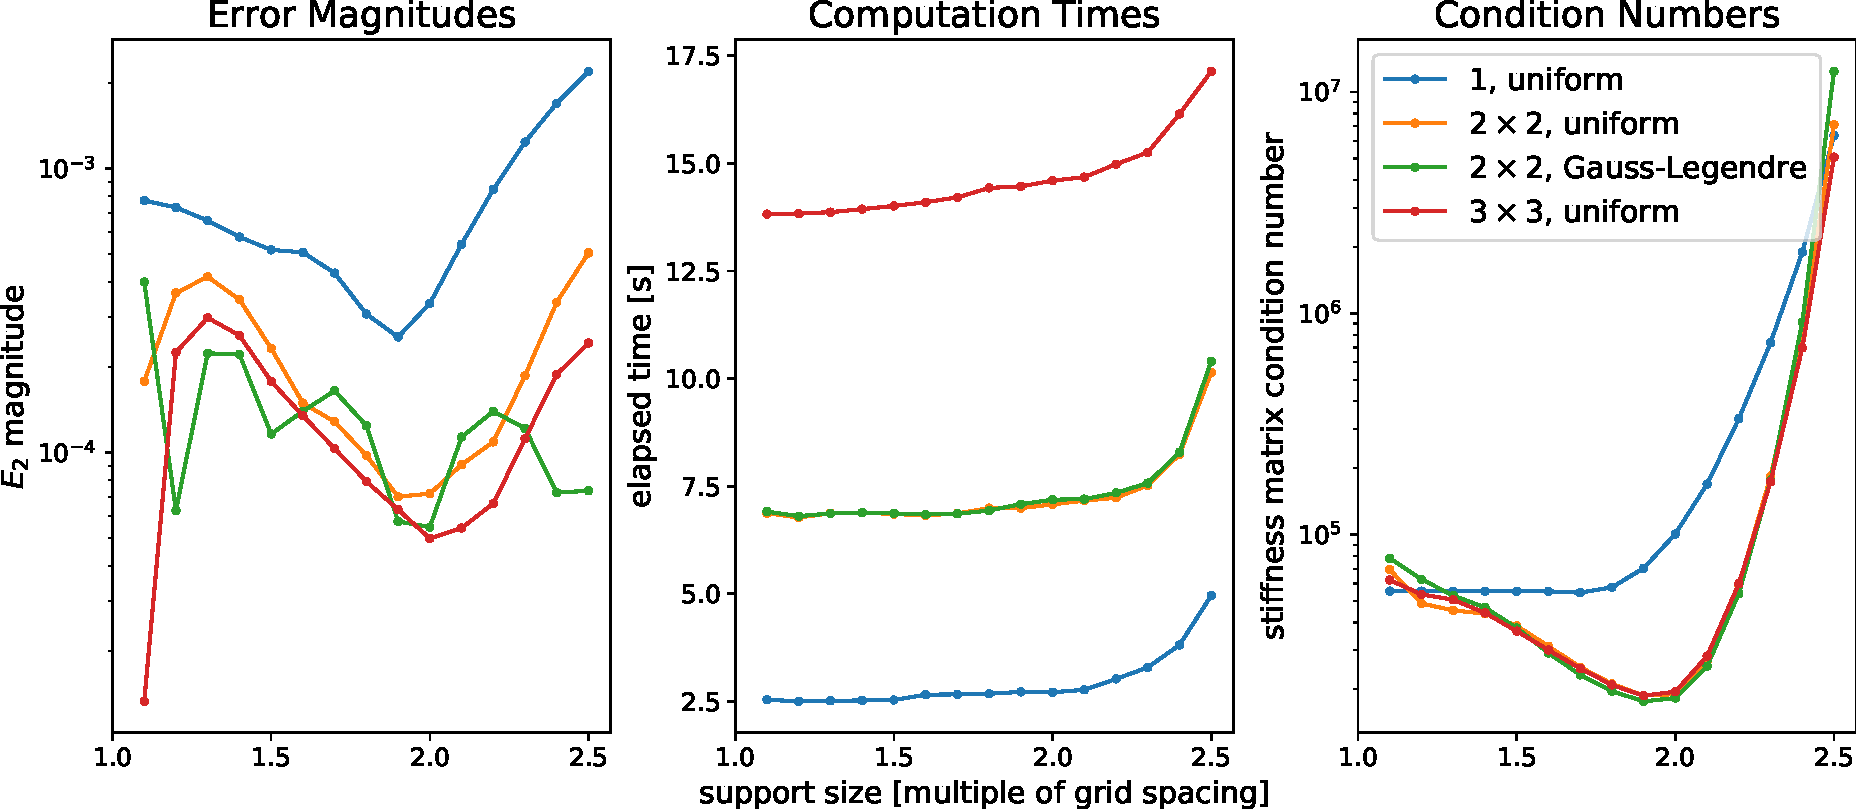
\includegraphics[width=\textwidth]{{../coursework-sam-maloney/MLS/MLS_timings_quadrature_1k}.pdf}
\caption{Comparison of minimum errors, simulation wall timings, and stiffness matrix condition numbers for the Galerkin assembly method using using different numbers and distributions of quadrature points. All values are for $N=64$ grid divisions and using cubic spline kernel weights.}
\label{fig:timings_quadrature_1k}
\end{figure}

As would be expected, the magnitude of the $E_2$ error norm decreases when moving from 1 point per cell to 4 points per cell, but the difference between 4 and 9 points per cell is quite marginal. Using a unform distribution of points throughout the domain produces errors that are more smoothly a function of the support size, compared to distributing the points according to Gauss-Legendre quadrature rules within each cell of the grid implied by the nodal point locations. The tested 4 point per cell Gauss-Legendre distribution outperforms even the 9 point per cell uniform distribution for some support sizes, but uderperforms both the 4 and 9 point per cell uniform distributions for others, although on average it outperforms the 4 point uniform distribution and is never much worse, making it arguably (albeit marginally) the preferred choice.

In terms of computational time, the 4 point per cell distributions take almost identical times, as expected, and average about 2.6X the runtime of the single point quadrature, with the 9 point per cell distribution taking about 2X as long again as the 4 point per cell distributions. Combined with the minimal decrease in error for the 9 point over the 4 point distributions (less than 2X in all cases except the leftmost point, which would probably be unadvisable from a robustness perspective for being to close to the size at which the shape function moment matrix becomes singular) the 9 point quadrature appears to be a poor choice for compuational efficiency.

The 4 point distirbutions on the other hand are much more interesting, as over most of the tested range the decrease in the error is greater than the 2.6X increase in the simulation time. Comparing this to decreasing the error by increasing the number of nodes, we see that since the assembly time and solution time are both expected to scale as $N^2$ and the method has been demonstrated to be 2nd order accurate ith regards to $N$, we would expect approximately 1:1 ratio between the decrease in error and increase in computational time when simply increasing the number of degrees of freedom. Since this ratio is seen to be greater than 1:1 in thse tests for the quadrature, it would appear that using a 4 point per cell quadrature is a computationally efficient way to increase the accuracy of the solution compared.


\section{Summary}

A very brief summary of the results:

\begin{itemize}
\item The Galerkin assembly method was found to be superior to the collocation method on essentially all counts.
\item Cubic splines slightly outperformed quartic splines as the kernel weighting functions, although the difference was marginal.
\item The method is very sensitive to the size of the support used, with too small supports leading to singlular moment matrices for the shape functions and too large supports leading to ill-conditioned system stiffness matrices.
\item For the quadrature in the Galerkin assembly method, using a 4 point per cell distribution was a computationally efficient way to improve accuracy, while using 9 points per cell was not.
\item Distributing the quadrature points according to Gauss-Legendre rules slightly outperformed a uniform distribution, although the difference was marginal and the Gauss-Legendre error had greater variance with respect to the support size.
\end{itemize}

\end{document}